\chapter{Interpolation und Kurvenanpassung}
%{\bf Learning goals:}
%\begin{itemize}
%\item Represent discrete data as functions to obtain function values apart from
%	the support points
%\item Increase presision at lower cost, i.e. few parameters together with
%	interpolating functions cover the whole space
%\item Fast numerical integration by using interpolated representations of
%	functions with a limited number of interpolating functions.
%\end{itemize}\newpage
\section{Diskrete Daten und Interpolationsfunktionen}
\subsection{Das Newton Polynom}\label{subsec:newton}
Gegeben eine funktion $f(x)$, die an einer endlichen Zahl von Punkten $x_i$ bekannt sei.
Wir haben $f(x_i)=y_i$.  Es seien $n+1$ Paare $P_i=(x_i,y_i)$ von Werten gegeben, die Stützstellen
Wir wollen uns eine pllynomiale Funktion n-ter Ordnung beschaffen, geschrieben als
\[p_n(x)=a_0+a_1 x+\dots +a_n x^n\]
für die
\[p_n(x_i)=a_0+a_1 x_i+\dots +a_n x_i^n=y_i\]
gilt. Das Newton'sche polynomoiale Approximationsschema ist das meistbenutzte,
da es unter anderem auch für irregulär verteilte Stützstellen funktioniert.
Darüberhinaus muss der Polynomgrad nicht a priori festgelegt werden.
\subsubsection{Dividierte Differenzen}
Dividierte Differenzen sind durch eine rekursive Division definiert. Sie sind sein nützliches Werkzeug, um die Koeffizienten von Interpolationspolynomen zu berechnen.
Für jede geordnete Folge von Stützstellen 
$x_k$, mit $k=0,1,\dots,n$ ist der Algorithmus zur Berechnung der dividierten Differenzen für eine Untermenge der Stützstellen gegeben als
\begin{eqnarray}
	\label{eq:divdiffs}
   D[x_i] f&=& f(x_i)=f_i, \qquad \nu \in \{ 0,\ldots,n\}\\
   D[x_i,x_j] f&=& \frac{f_j-f_i}{x_j-x_i}\nonumber\\
   D[x_i,x_j,x_k] f&=& \frac{D[x_j,x_k]f-D[x_i,x_j]f}{x_k-x_i}\nonumber\\
   D[x_i,x_j,\ldots,x_l,x_m] f&=& \frac{D[x_j,\dots,x_m]f-D[x_i,\dots,x_l]f}{x_m-x_i}\nonumber
\end{eqnarray} 
Manchmal ist ed bequemer die folgende Matrixnotation zu benutzen
\begin{equation} 
	D_{i,j}=D[x_i,x_{i+1},\dots,x_{i+j}]f
	\label{eq:invdivdiffs}
\end{equation}
\subsubsection{Berechnung der Newton'schen Form}
Wir wollen $f(x)\approx p_n(x)$ finden, wobei $p_n(x)$ ein Newton'sches Polynom
ist, gegeben durch die Punkte $(x_0,f_0),\dots,(x_n,f_n)$, das folgendermaßen
definiert sei
\begin{equation}
	p_n(x)=f_0+(x-x_0)D[x_0,x_1]f+\dots +(x-x_0)\cdots (x-x_{n-1})D[x_0,\dots,x_n]f
	\label{eq:newtonpoly}
\end{equation}
oder mit der oben erwähnten Matrixform der dividierten Differenzen
\[
p_n(x)=D_{0,0}+D_{0,1}(x-x_0)+\dots +D_{0,n}(x-x_0)\cdot(x-x_{n-1})=D_{0,0}+\sum_{k=1}^nD_{0,k}\prod_{j=0}^{k-1}(x-x_j)
\]
Der größte Vorteil der hier präsentierten Methode ist, dass die dividierten Differenzen 
$D_{i,k}$ eng mit der k-ten Ableitung am Punkt $i$ verbunden sind.  Es ist
hiermit möglich zu entscheiden, ob eine Funktion, die durch ein Anzahl von
Stützstellen gegeben ist,  durch ein Polynom k-terOrdnung approximierbar ist.  Anders
gesagt, wenn alle Koeffizienten der  Matrixform der dividierten Differenzen in
der k-ten Spalte von derselben Größenordnung sind, d.h.  $D_{0,k}\approx
D_{0,1}\approx D_{0,2}\approx\dots$.
\subsection{Lagrangeinterpolation}
Lagrangepolynome sind so konstruiert, dass Sie durch alle Stützstellenpunkte, wie in \ref{subsec:newton}, gehen.
\[
L_i(x)=\prod_{j=0,j\neq i}^n\frac{(x-x_j)}{x_i-x_j}=\frac{(x-x_0)\ldots(x-x_{i-1})(x-x_{i+1})\ldots(x-x_n)}{(x_i-x_0)\ldots(x_i-x_{i-1})(x_i-x_{i+1})\ldots(x_i-x_n)}
\]
Wie man leicht sieht ist
\[
L_i(x)=\left\{
\begin{array}{rcl}
1&\mbox{ für }&x=x_i\\ 
0&\mbox{ für }&x=x_{j\ne i}
\end{array}\right.
\]
oder in Anderen Worten $L^n_j(x_i)=\delta_{ij}$. Das Polynom, das durch die 
$n+1$ Interpolationspunkte geht, schreibt man
\[ p_n(x)=\sum_{i=0}^n y_i\ L_i(x) \]
\subsubsection{Alternative Form  der Langrangeinterpolationsformeln}
Dieses Polynom stimmt mit der Funktion $f(x)$ an den Abszissen der Interpolationspunkte $x_i$ exakt überein. Neben $x_i$ tritt i. A. ein Fehler auf, der aber bestimmbar ist. Wir schreiben das Polynom um
\[ p_n(x)=\sum_{i=0}^n y_i\ \prod_{j=0,j\neq i}^n\frac{x-x_j}{x_i-x_j}=
\sum_{i=0}^n y_i 
\underbrace{
\frac{1}{x-x_i} \prod_{j=0,j\neq i}^n\frac{1}{x_i-x_j} 
}_{\mu_i}\ 
\underbrace{\prod_{k=0}^n (x-x_k)}_{l(x)}
\]
Es gibt eine alternative Schreibweise für das Polynom
\begin{equation}\label{eq:1stbarycentric}
	p_n(x) = l(x)\sum_{i=0}^n \mu_iy_i,
\end{equation}
gemeinhin als baryzentrische Interpolationsformel bezeichnet. Wenn wir verlangen, dass $p_n(x)=1$ sehen wir, dass $y_i=1$ und deshalb haben wir
\[ 1 = l(x)\sum_{i=0}^n \mu_i \]
Teilen wir (\ref{eq:1stbarycentric}) durch letzteres, dann erhalten wir die zweite baryzentrische Form
\begin{equation}
	p^n(x)=\frac{\sum_{i=0}^n \mu_iy_i}{\sum_{i=0}^n \mu_i}
	\label{eq:2ndbarycentric}
\end{equation}
%The $n+1$ Lagrange polynomials of order n add up to unity everywhere in the interval.
\subsubsection{Interpolationspunkte gleichen Abstands}
Für Interpolationspunkte gleichen Abstands $x_i-x_{i-1}=h$ erhalten wir
\begin{eqnarray*}
\lambda_i =\prod_{j=0,j\neq i}^n\frac{1}{x_i-x_j} 
&=&\frac{1}{(-1)^{n-i}h^n(i(i-1)(i-2)\ldots1)(1\ 2\ \ldots\ (n-1))}\\[1ex]
&=&\frac{(-1)^{n-i}}{h^n n!}
\left(\begin{array}{c}n\\ i\end{array}\right)
\end{eqnarray*}
In diesem Fall können wir  
\[
\mu_i=\frac{1}{x-x_i} \prod_{j=0,j\neq i}^n\frac{1}{x_i-x_j}=
\frac{1}{x-x_i} \lambda_i
\]
schreiben. Wenn wir beachten, dass in (\ref{eq:2ndbarycentric}) alle Faktoren
im Zaähler und Nenner, über die nicht summiert wird, sich wegheben, dann
erhalten wir die einfache Form
\[ 
  \lambda_i^* = (-1)^i\left(\begin{array}{c}n\\ i\end{array},\right)
\]
die $\lambda_i$ für unregelmäßige Abstände der Interpolationspunkte ersetzt..
\subsubsection{Application of Lagrange polynomials}
For a given number of sample points let us calculate the derivative of the
Lagrange polynomial, to read
\[ 
\frac{d^n p_n(x)}{dx^n}=\sum_{i=0}^ny_i\lambda_in!\approx f^{(n)}(x)
\]
The latter is an approximation for the derivative of the interpolated function.
We consider an equidistant set of sample points $x_i=x_{i-1}+h,\ \ \ x_i=x_0+i
h$ and an interpolation of second order, which reads
\[
~p_2(x)=\frac{1}{2h^2}
\left( y_0(x-x_1)(x-x_2)
     -2y_1(x-x_0)(x-x_2)
      +y_2(x-x_0)(x-x_1)\right)
\]
Its derivative reads
\[
p_2'(x)=\frac{1}{2h^2}
\left( y_0(2x-x_1-x_2)
     -2y_1(2x-x_0-x_2)
      +y_2(2x-x_0-x_1) \right)
\]
Thus we have the approximations for the derivatives at the sample points given
as
\begin{equation}\label{eq:leftderiv} 
f'(x_0)\approx\frac{1}{2h}\left({-3y_0+4y_1-y_2}\right)
\end{equation}
\begin{equation}\label{eq:centerderiv}
f'(x_1)\approx\frac{1}{2h}\left({-y_0+y_2}\right)
\end{equation}
\begin{equation}\label{eq:rightderiv}
f'(x_2)\approx\frac{1}{2h}\left({-y_0+4y_1-2y_2}\right)
\end{equation}
\subsubsection{Alternate formulation}
Let us use the alternate formulation for equidistant sample points. For
the $\lambda_i$ and $\mu_i$ we have 
\begin{eqnarray*}
\lambda_0&=&\frac{1}{(x_1-x_0)(x_2-x_0)}=\frac{1}{2h^2}\\
\lambda_1&=&\frac{1}{(x_0-x_1)(x_2-x_1)}=-\frac{1}{h^2}\\
\lambda_2&=&\frac{1}{(x_0-x_2)(x_1-x_2)}=\frac{1}{2h^2}
\end{eqnarray*}
and
\begin{eqnarray*}
\mu_0&=&\lambda_0\frac{1}{(x-x_0)}=\frac{1}{2h^2 (x-x_0)}\\
\mu_1&=&\lambda_1\frac{1}{(x-x_1)}=-\frac{1}{h^2 (x-x_1)}\\
\mu_2&=&\lambda_2\frac{1}{(x-x_2)}=\frac{1}{2h^2 (x-x_2)}
\end{eqnarray*}
While the reduced quantities read
\begin{eqnarray*}
\lambda^*_0&=&(-1)^0\left(\begin{array}{c}2 \\ 0\end{array}\right)=1\\
\lambda^*_0&=&(-1)^1\left(\begin{array}{c}2 \\ 1\end{array}\right)=-2\\
\lambda^*_0&=&(-1)^2\left(\begin{array}{c}2 \\ 2\end{array}\right)=1
\end{eqnarray*}
and
\begin{eqnarray*}
\mu_0^*&=&\lambda_0^*\frac{1}{(x-x_0)}=\frac{1}{(x-x_0)}\\
\mu_1^*&=&\lambda_1^*\frac{1}{(x-x_1)}=-\frac{2}{(x-x_1)}\\
\mu_2^*&=&\lambda_2^*\frac{1}{(x-x_2)}=\frac{1}{(x-x_2)}
\end{eqnarray*}
And finally we obtain
\[
p_2(x)=\frac{\displaystyle\sum_{i=0}^2 \mu_iy_i}{\displaystyle\sum_{i=0}^n \mu_i}
=\frac{(x-x_1) (x-x_2) y_0 -2(x-x_0) (x-x_2) y_1+ (x-x_0) (x-x_1) y_2}{2h^2}
\]
\subsection{Interpolation by continued fraction}
Some functions $f(x)$ cannot be approximated well by polynoms, since they
contain horizontal or vertical aymptotes. In these cases it is convenient to
approximate $f(x)$ by a limited continued fraction.

It is possible to expand $f(x)$ in a continuous fraction provided one can write
\begin{equation}
	f(x)=y_0+\cfrac{x-x_0}{y_1+\cfrac{x-x_1}{y_2+\cfrac{x-x_2}{y_3+\cdots}}}
	\label{eq:contfrac}
\end{equation}
The expansion given in (\ref{eq:contfrac}) is limited to a finite order for
practical reasons, i.e.\ it is a truncated continuous fraction. $f(x)$ is known
through its values $f_j=f(x_j)$ at the support points $x_j$, with
$j=0,1,\dots,n$. The $y_k$ may be expressed by means of the inverse divided
differences $d_{ij}$, which are given by
\begin{eqnarray}
	d_{i,0}f&=&f_i\mbox{, for }i=0,\dots,n\nonumber\\
	d_{i,1}f&=&\frac{x_{i+1}-x_i}{f_{i+1}-f_i}\mbox{, for }i=0,\dots,n-1\label{eq:invdivdif}\\
	d_{i,j}f&=&\frac{x_{i+1}-x_i}{f_{i+1}-f_i}+d_{i+1,j-2}f\mbox{, for }j=2,\dots,n\mbox{ and }i=0,\dots,n-j\nonumber
\end{eqnarray}
Thus we have 
\[
y_0=f_0,\ y_1=d_{0,1}f,\ y_k=d_{0,k}f-d_{0,k-2}\mbox{ with }2\le k\le n
\]
Having calculated the values $y_0,y_1,\dots,y_n$ we obtain a continuos fraction
truncated at the term $(x-x_{n-1}/y_n$, that allows to calculate an
interpolated value of $f$ at $x$ through the recursive relation
\begin{eqnarray*}
	F_n(x)&=&y_n\\
	F_k(x)&=&y_k+\frac{x-x_k}{F_{k+1}(x)}\mbox{ with }k=n-1\mbox{ to }0\\
	f(x)&=&F_0(x)
\end{eqnarray*}

\begin{example}{Interpolation}
	\label{ex:contfrac}
Interpolate at $x=3.5$ the function $f(x)$ given through
\begin{center}
\begin{tabular}{c|rrrrr}
	$x_i$&-2&0&2&3&4\\\hline
	$f_i$&2&0&-10&-33&-124
\end{tabular}
\end{center}
Applying the above algorithm (verify!) we find the expansion
\begin{equation}
f(x)=-124+\cfrac{x-4}{\frac{-1}{91}+\cfrac{x-3}{\frac{5187}{34}+\cfrac{x-2}{\frac{680}{3913}+\cfrac{x}{\frac{-903}{34}}}}}
	\label{eq:excontfrac}
\end{equation}
\end{example}

\subsection{Spline interpolation}
A spline is a thin wood or metal strip used in building construction. The most
useful spline functions follow the same constraints as bent metal or wooden
strips, they tend to minimize curvature. Our starting point is again the set of
collocation points $(x_i,y_i)$. We are looking for a function $sp(x_i)=y_i$
that connects all the collocation points and that respects certain constraints.
Linear connections between the collocation points are simple traverses of
linear functions that connect the collocation points. The only constraints that
seem to make sense in this case are that the endpoints of the lines go through
the collocation points. If we allow higher order polynomial functions to connect
the sample points, we might ask for more complicated constraints to be
respected. A spline ist a set of polynomes of 3rd degree that connect the
collocation points. Our task will be to find the coefficients of the single
polynomes, given the constaints.

Assume that we want to minimize the overal bending energy of the spline, given by
\begin{equation}
	S=\int_{x_0}^{x_n}\left(\frac{d^2 s(x)}{dx^2}\right)^2dx
	\label{eq:bendingE}
\end{equation}
This is equivalent to the requirement that the variation $\delta S$ of $S$ vanishes, i.e.
\begin{equation}
	\delta S=\int_{x_0}^{x_n} s''(x) \delta s''dx=0
	\label{eq:Evar}
\end{equation}
We divide the integral in intervals given by the positions of the collocation points
\begin{equation}
	\delta S=\sum_{i=0}^{n-1}\int_{x_i}^{x_{i+1}} s''(x) \delta s''dx=0
	\label{eq:Evarint}
\end{equation}
At the supports the variation $\delta s''(x_j)=0$.

In order to solve for the coefficients of the set of polynomes, let us
transform (\ref{eq:Evarint}) with the help of partial integration.

\begin{note}{} 
	Partial integration means $\int f\ dg = f\cdot g - \int g\ df$.
\end{note}

We have
\[
\int_{x_{i-1}}^{x_i}s''(x)\delta s'' (x) dx=\int_{x_{i-1}}^{x_i}s''(x)d(\delta s' (x))= \left. {s''(x)\delta s'(x)}\right|_{x_{i-1}}^{x_i}-\int_{x_{i-1}}^{x_i}\delta s' (x)d(s''(x))
\]
\begin{eqnarray*}
\int_{x_{i-1}}^{x_i}\delta s' (x)d(s''(x))=\int_{x_{i-1}}^{x_i}s'''(x)\delta s' (x)dx&=&
\int_{x_{i-1}}^{x_i}s'''(x)d(\delta s(x))\\[1ex]
&=&\left. {s'''(x)\delta s(x)}\right|_{x_{i-1}}^{x_i}-\int_{x_{i-1}}^{x_i} \delta s(x) d(s'''(x))
\end{eqnarray*}
\[
\int_{x_{i-1}}^{x_i} \delta s(x) d(s'''(x))=\int_{x_{i-1}}^{x_i} s''''(x)\delta s(x) dx
\]
It is
\[
d(s'''(x))= \frac{d(s'''(x))}{dx}dx= s''''(x) dx
\]
The variation of the integral (\ref{eq:Evarint})
finally reads
\begin{eqnarray*}
\sum_{i=1}^n\int_{x_{i-1}}^{x_i}s''(x)\delta s'' (x)dx
&=&\sum_{i=1}^n\left(\left. s''(x)\delta s'(x)\right|_{x_{i-1}}^{x_i}-\left.
s'''(x)\delta s(x)\right|_{x_{i-1}}^{x_i}\right. \\[1ex]
&&\left. -\int_{x_{i-1}}^{x_i} s''''(x)\delta s(x)dx\right)
\end{eqnarray*}
Remember that this must hold for arbitrary variations $\delta$ - besides at $x_0$ and $x_n$ where $\delta s=0$ holds - and thus their coefficients must vanish. 
\begin{eqnarray*}
s''''(x)&=&0 \text{ for } x\neq x_i
\\
s''(x_0)&=&s''(x_n)=0
\\
s''(x_i)^+&=&s''(x_i)^-,\ \ \ i=1,2,\ldots,n-1
\end{eqnarray*}

Consider the interval $[x_i,x_{i+1}]$ where $h_i=x_{i+1}-x_i$. The coefficients
of the cubic polynomial
\[ a_i(x)=a_i(x-x_i)^3+b_i(x-x_i)^2+c_i(x-x_i)+d_i \]
are to be determined. Compute the value of the polynomial and its first and
second derivatives at each of the two endpoints to give
\begin{eqnarray}
	  a_i&=&\frac{1}{6h_i}(y^{\prime\prime}_{i+1}
	        -y^{\prime\prime}_{i})\label{eq:splinecoefai} \\
	  b_i&=&\frac{1}{2} y^{\prime\prime}_{i}\label{eq:splinecoefbi}\\
	  c_i&=&\frac{1}{h_i}(y_{i+1}-y_i)-\frac{1}{6}h_i (y^{\prime\prime}_{i+1}
	        -y^{\prime\prime}_{i})\label{eq:splinecoefci}\\
	  d_i&=&y_i\label{eq:splinecoefdi}
  \end{eqnarray}
Thus in all intervals we have related the coefficients of the repective polynom
to the second derivative at the endpoints of the interval
(\ref{eq:splinecoefai}-\ref{eq:splinecoefdi}). The final task is to find an equation system to solve
for the $y_i''$.

\begin{example}{Spline interpolation on 5 intervals}
	\begin{eqnarray*}
		\lefteqn{\left(
		\begin{array}{cccc}
			2(h_0+h_1)&h_1&0&0\\
			h_1&2(h_1+h_2)&h_2&0\\
			0&h_2&2(h_2+h_3)&h_3\\
			0&0&h_3&2(h_3+h_4)
		\end{array}
		\right)\cdot
		\left(
		\begin{array}{c}
			y^{\prime\prime}_1\\
			y^{\prime\prime}_2\\
			y^{\prime\prime}_3\\
			y^{\prime\prime}_4
		\end{array}
		\right)
		=}\hspace{7cm}\\
		&&\left(
		\begin{array}{c}
			\frac{6}{h_0}(y_1-y_0)+\frac{6}{h_1}(y_2-y_1)+h_0y_0^{\prime\prime}\\
			\frac{6}{h_1}(y_2-y_1)+\frac{6}{h_2}(y_3-y_2)\\
			\frac{6}{h_2}(y_3-y_2)+\frac{6}{h_3}(y_4-y_3)\\
			\frac{6}{h_3}(y_4-y_3)+\frac{6}{h_4}(y_5-y_4)+h_4y_5^{\prime\prime}
		\end{array}
		\right)
	\end{eqnarray*}
\end{example}

\subsection{Bernstein Polynomials}
Any interval $[a,b]$ can be mapped to the unit interval $[0,1]$ by the transformation
\[
\lambda=(t-a)/(b-a)
\]
The Bernstein basis polynomials are defined on the unit interval as
\begin{equation}
	 b_{\nu,n}(x) = \binom{n}{\nu} x^{\nu} (1-x)^{n-\nu}, \qquad \nu=0,\ldots,n. 
	\label{eq:Bernsteinbasis}
\end{equation}
They show important properties that will be used for B\'ezier splines. The
Berstein basis polynomials of same order $n$ add up to unity. This can be seen
very easily. Look at the following term
\[ 1=\left(x+(1-x)\right)^n=\sum_{i=0}^n \binom{n}{i} x^i(1-x)^{n-i}\]
The right hand side is the sum over the Bernstein basis polynomials of the same
order $n$.
\begin{figure}[!ht]
\begin{center}
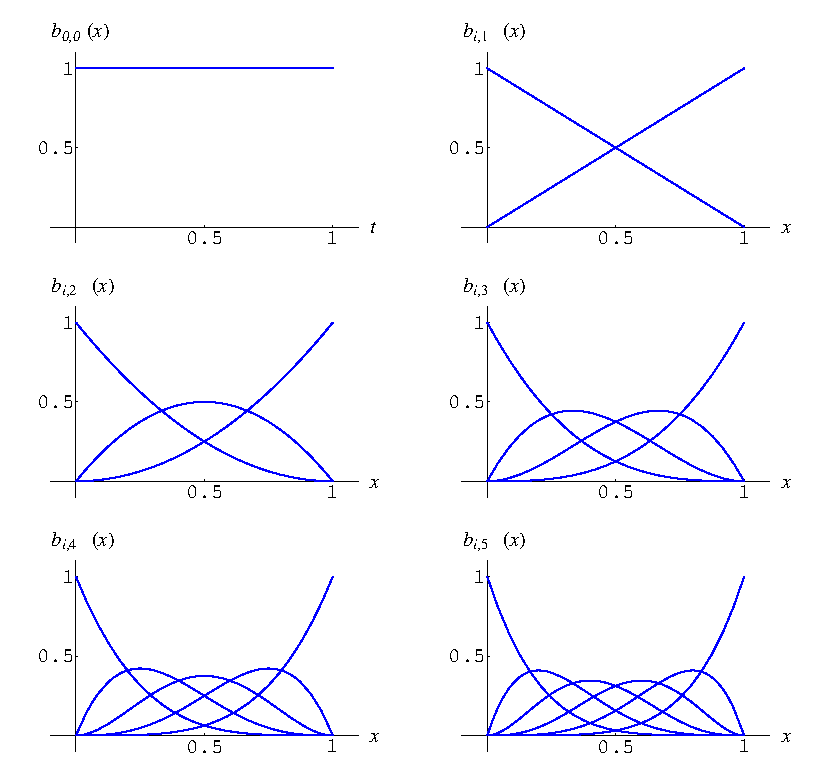
\includegraphics[width=\textwidth]{fig/BernsteinPol}
\caption{The Bernstein polynomials up to order $n=5$.\label{fig:BerPol}}
\end{center}
\end{figure}
\subsection{B\'ezier splines}
B\'ezier splines are curves defined on an interval for a parameter $t\in [0,1]$.
They are controlled by points that contribute to the curve parametrized by $t$
with a fixed weighting function in $t$. Two point, e.g., produce a straight
line, a so called linear B'ezier curve, to read
\[     \mathbf{B}(t)=\mathbf{P}_0 + t(\mathbf{P}_1-\mathbf{P}_0)=(1-t)\mathbf{P}_0 + t\mathbf{P}_1 \mbox{ , } t \in [0,1] \]
A cubic B\'ezier spline reads
\[     \mathbf{B}(t)=(1-t)^3\mathbf{P}_0+3(1-t)^2t\mathbf{P}_1+3(1-t)t^2\mathbf{P}_2+t^3\mathbf{P}_3 \mbox{ , } t \in [0,1]\]
A B\'ezier curve of degree $n$ reads
\[ \mathbf{B}(t)=\sum_{i=0}^n \binom{n}{i}(1-t)^{n-i}t^i\mathbf{P}_i =(1-t)^n\mathbf{P}_0+\binom{n}{1}(1-t)^{n-1}t\mathbf{P}_1+\cdots+t^n\mathbf{P}_n \mbox{ , } t \in [0,1]\]
Observe that in order to adjust the path the curve must follow you have to move
the control points. The extension to surfaces is straight forward
\[ x(s,t)=\sum_{i=0}^n \sum_{j=0}^m B_i^n(s) \; B_j^m(t) \; \mathbf{k}_{i,j}\]
where the $B_i^n(\nu)$ are the Bernstein polynomials and the $\mathbf{k}_{i,j}$ are the $(n+1)(m+1)$ control points.
\subsection{Legendre Polynomials}
Legendre polynomials are defined as
\begin{equation}
	    P_n(x) = \frac{1}{2^n n!}\frac{d^n}{dx^n } \left[ (x^2 -1)^n \right]
	\label{eq:legendre}
\end{equation}
They derive from the solution of the following differential equation
\[\frac{d}{dx} \left[ (1-x^2)\frac{d}{dx} P_n(x) \right] + n(n+1)P_n(x) = 0\]
Legendre polynomials are orthogonal on the interval $[-1,1]$, i.e.
\[     \int_{-1}^{1} P_m(x) P_n(x)\,dx = \frac{2}{2n + 1} \delta_{mn} \]
holds.

The first six Legendre polynomials read
\begin{eqnarray*}
 	P_0(x)=1\\
	P_1(x)=x\\
	P_2(x)=\frac{1}{2} (3x^2-1) \\
	P_3(x)=\frac{1}{2} (5x^3-3x) \\
	P_4(x)=\frac{1}{8} (35x^4-30x^2+3)\\
	P_5(x)=\frac{1}{8} (63x^5-70x^3+15x)
\end{eqnarray*}
\newpage
\section{Least square fit}
Suppose you are given a set of date $z_i\in\{Z\}$ measured at points $x_i$ and $y_i$. We want to find a function $f(x,y;\mathbf{p})$ which depends on a vector $\mathbf{p})$ of paramters $p_k$. Assume that $f(x=0,y=0)=0$. Thus we propose a polynomial function $f(x,y;\mathbf{p})=p_0\cdot x+p_1\cdot y+p_2\cdot x^2+p_3\cdot x\cdot y+p_4\cdot y^2$ the data set of measurements $\{x_i,y_i,z_i\}$ we want to fit to. We choose a least square method, i.e.
\[
\sum_i \left( f(x_i,y_i;\mathbf{p})-z_i\right)^2 = \text{Min}.
\]
Which in turn is equivalent to require
\[
\frac{\partial}{\partial p_k}\sum_i \left( f(x_i,y_i;\mathbf{p})-z_i\right)^2=\sum_i \left( f(x_i,y_i;\mathbf{p})-z_i\right)\frac{\partial}{\partial p_k}f(x_i,y_i;\mathbf{p})=0
\]
this yields a linear system of equation for the $p_k$ to read
\begin{align*}
p_0\sum_i x_i^2+p_1\sum_i x_i\cdot y_i+p_2\sum_i x_i^3+p_3\sum_i x_i^2\cdot y_i+p_4\sum_i x_i\cdot y_i^2&=\sum_iz_i\cdot x_i\\
p_0\sum_i x_i\cdot y_i+p_1\sum_i y_i^2+p_2\sum_i x_i^2\cdot y_i+p_3\sum_i x_i\cdot y_i^2+p_4\sum_i y_i^3&=\sum_iz_i\cdot y_i\\
p_0\sum_i x_i^3+p_1\sum_i x_i^2\cdot y_i+p_2\sum_i x_i^4+p_3\sum_i x_i^3\cdot y_i+p_4\sum_i x_i^2\cdot y_i^2&=\sum_iz_i\cdot x_i^2\\
p_0\sum_i x_i^2\cdot y_i+p_1\sum_i x_i\cdot y_i^2+p_2\sum_i x_i^3\cdot y_i+p_3\sum_i x_i^2\cdot y_i^2+p_4\sum_i x_i\cdot y_i^3&=\sum_iz_i\cdot x_i\cdot y_i\\
p_0\sum_i x_i\cdot y_i^2+p_1\sum_i y_i^3+p_2\sum_i x_i^2\cdot y_i^2+p_3\sum_i x_i\cdot y_i^3+p_4\sum_i x_i\cdot y_i^4&=\sum_iz_i\cdot y_i^2
\end{align*}
Let us write this as a 
\[
\mathbf{A}\cdot\mathbf{p}=\mathbf{b}
\]
Note that $\mathbf{A}$ is symmetric and the matrix entries read
\[ 
\mathbf{A}=
\begin{pmatrix}
\sum_i x_i^2&\sum_i x_i\cdot y_i&\sum_i x_i^3&\sum_i x_i^2\cdot y_i&\sum_i x_i\cdot y_i^2\\
\sum_i x_i\cdot y_i&\sum_i y_i^2&\sum_i x_i^2\cdot y_i&\sum_i x_i\cdot y_i^2&\sum_i y_i^3\\
\sum_i x_i^3&\sum_i x_i^2\cdot y_i&\sum_i x_i^4&\sum_i x_i^3\cdot y_i&\sum_i x_i^2\cdot y_i^2\\
\sum_i x_i^2\cdot y_i&\sum_i x_i\cdot y_i^2&\sum_i x_i^3\cdot y_i&\sum_i x_i^2\cdot y_i^2&\sum_i x_i\cdot y_i^3\\
\sum_i x_i\cdot y_i^2&\sum_i y_i^3&\sum_i x_i^2\cdot y_i^2&\sum_i x_i\cdot y_i^3&\sum_i x_i\cdot y_i^4
\end{pmatrix},
\]
while we habe for the r.h.s. of the linear system
\[ 
\mathbf{b}=
\begin{pmatrix}
\sum_iz_i\cdot x_i\\
\sum_iz_i\cdot y_i\\
\sum_iz_i\cdot x_i^2\\
\sum_iz_i\cdot x_i\cdot y_i\\
\sum_iz_i\cdot y_i^2
\end{pmatrix},
\]
$\mathbf{A}$ and $\mathbf{b}$ can be easily calculated and thus we have $\mathbf{p}=\mathbf{A}^{-1}\cdot\mathbf{b}$. The only task left is to find an analytical expression for the inverse of $\mathbf{A}$, which components read
\[
\mathbf{A}^{-1}_{ij}=\frac{\alpha_{ij}}{|\mathbf{A}|},
\]
where the $\alpha_{ij}$ are the elements of the adjoint matrix $\mathbf{A}_{ad}$. 
\begin{note}{The adjoint matrix elements}
\[
\alpha_{ij}=(-1)^{i+j}
\left|
\begin{matrix}
a_{11}&\dots &a_{1,j-1}& &a_{1,j+1}&\dots &a_{1n}\\
a_{11}&\dots &a_{1,j-1}& &a_{1,j+1}&\dots &a_{1n}\\
&&&\vdots &&&\\
a_{11}&\dots &a_{1,j-1}& &a_{1,j+1}&\dots &a_{1n}\\
a_{11}&\dots &a_{1,j-1}& &a_{1,j+1}&\dots &a_{1n}\\
\end{matrix}
\right|\text{, where }a_{ij}=(\mathbf{A})_{ij}
\]
\end{note}